%% chapter1_slides.tex
%% Beamer slides for Chapter 1: Introduction
%% "Hypothesis Testing with E-Values" by Aaditya Ramdas and Ruodu Wang (arXiv:2410.23614)
%% Reader-friendly style: complete sentences, symbol explanations, worked examples.
%% Compiled with: pdflatex -interaction=nonstopmode chapter1_slides.tex  (twice)
\documentclass[aspectratio=169,10pt]{beamer}

\usetheme{Madrid}
\usecolortheme{seahorse}
\usefonttheme{professionalfonts}

%% ── Packages ──────────────────────────────────────────────────────────────
\usepackage{amsmath,amssymb,amsfonts}
\usepackage{mathtools}
\usepackage{graphicx}
\usepackage{booktabs}
\usepackage{xcolor}
\usepackage{listings}

\graphicspath{{figures/}}

%% ── Python listing style ─────────────────────────────────────────────────
\lstdefinestyle{pycode}{
  language=Python,
  basicstyle=\ttfamily\scriptsize,
  numbers=left,
  numberstyle=\tiny\color{gray},
  frame=single,
  backgroundcolor=\color{gray!7},
  keywordstyle=\color{blue!70!black}\bfseries,
  commentstyle=\color{green!50!black}\itshape,
  stringstyle=\color{orange!80!black},
  showstringspaces=false,
  breaklines=true,
  tabsize=2,
  xleftmargin=1.0em,
  framexleftmargin=1.0em,
  aboveskip=4pt,
  belowskip=4pt,
}
\lstset{style=pycode}

%% ── Metadata ─────────────────────────────────────────────────────────────
\title[E-Values -- Ch.1]{Hypothesis Testing with E-Values}
\subtitle{Chapter 1: Introduction}
\author{Based on Ramdas \& Wang}
\institute{arXiv:2410.23614}
\date{}

\setbeamertemplate{footline}[frame number]
\setbeamertemplate{navigation symbols}{}

%% ══════════════════════════════════════════════════════════════════════════
\begin{document}

\begin{frame}
  \titlepage
\end{frame}

\begin{frame}{Chapter Overview}
  \tableofcontents
\end{frame}

%% ══════════════════════════════════════════════════════════════════════════
\section{Notation you'll need}
%% ══════════════════════════════════════════════════════════════════════════

\begin{frame}[allowframebreaks]{Notation You'll Need for This Chapter}

Before diving in, here is a plain-English glossary of every non-elementary
term and symbol used later in this deck. Nothing here requires measure
theory --- treat each analogy as the working definition you need.

\begin{itemize}
  \item \textbf{Null hypothesis, $\mathcal{P}$}: the ``boring'' explanation of
    the data we test against -- a \emph{set} of candidate probability
    distributions (e.g., ``the coin is fair,'' i.e., $\{\text{Bernoulli}(0.5)\}$).
  \item \textbf{Alternative hypothesis, $\mathcal{Q}$}: the ``interesting''
    explanation we'd like evidence for (e.g., ``the coin is biased towards
    heads'').
  \item \textbf{$\mathbb{P}, \mathbb{Q}$}: a single probability distribution;
    $\mathbb{P}\in\mathcal{P}$ means $\mathbb{P}$ is one specific member of
    the null hypothesis set.
  \item \textbf{Simple vs.\ composite hypothesis}: simple means the set has
    exactly one distribution (e.g., $\{\mathbb{P}\}$); composite means it has
    more than one (e.g., ``$\theta \neq 0.5$'' covers infinitely many biased
    coins).
  \item \textbf{Random variable $X$}: a quantity whose value depends on
    the random outcome (here: our data).
  \item \textbf{$\mathbb{E}^{\mathbb{P}}[X]$}: the expectation (long-run
    average) of $X$, computed \emph{assuming} $\mathbb{P}$ is the true
    distribution.

\framebreak

  \item \textbf{E-variable / e-value}: a nonnegative random variable $E$
    with $\mathbb{E}^{\mathbb{P}}[E]\le 1$ under every null distribution.
    Analogy: a bet that is never favorable to you (on average) if the null
    is true, but pays off big if the null is false. ``E-value'' is the
    number you actually observe.
  \item \textbf{P-variable / p-value}: you already know this one --- a
    number in $[0,1]$ that is uniform-or-larger under the null. Small
    p-value = evidence against the null. (\emph{Opposite} convention to
    e-values: for e-values, \emph{large} is evidence against the null.)
  \item \textbf{Test $\phi$}: a (possibly randomized) decision rule taking
    values in $[0,1]$, interpreted as ``the probability I reject $H_0$.''
    A \textbf{binary} test only ever outputs 0 (``don't reject'') or 1
    (``reject'').
  \item \textbf{Type-I error / level $\alpha$}: the chance of a false alarm
    (rejecting a true null). A ``level-$\alpha$ test'' controls this chance
    to be at most $\alpha$ (e.g., $\alpha = 0.05$).
  \item \textbf{Likelihood ratio $\mathrm{d}\mathbb{Q}/\mathrm{d}\mathbb{P}$}:
    for a data point $x$, how much more likely $x$ is under $\mathbb{Q}$
    than under $\mathbb{P}$. If data are continuous/discrete with densities
    (or probability mass functions) $q(x), p(x)$, this is just $q(x)/p(x)$.

\framebreak

  \item \textbf{Exact e/p-variable}: one where the defining inequality is
    always an equality ($\mathbb{E}^{\mathbb{P}}[E]=1$, or
    $\mathbb{P}(P\le\alpha)=\alpha$) --- the ``tightest possible'' case.
  \item \textbf{Stochastically larger}: random variable $X$ is stochastically
    larger than a reference distribution if $X$ is, loosely, ``at least as
    likely to be big.'' (Formally: its cdf is never above the reference cdf.)
  \item \textbf{Supermartingale idea (informal)}: a wealth process that, on
    average, never grows from one step to the next given the past --- like
    a casino game that is fair or tilted against you. We will only need the
    intuition, not the formal machinery.
  \item \textbf{Filtration / adapted / stopping time (informal)}: think of a
    filtration as ``the information you've seen up to now, growing over
    time''; a process is adapted if, at each time, it only uses information
    seen so far; a stopping time is a rule for ``when to stop'' that only
    looks at data observed up to that moment (no peeking into the future).

\framebreak

  \item \textbf{E-process}: a sequence of e-values $E_1, E_2, \dots$ (built
    up as data arrive) that remains a valid e-value \emph{even if you stop
    early}, at any data-dependent stopping time. This is what lets e-values
    handle ``peeking'' safely.
  \item \textbf{Exchangeable}: a collection of random variables whose joint
    behavior does not change if you relabel/permute them -- e.g., shuffling
    a deck of otherwise-identical-looking cards.
  \item \textbf{Calibrator}: a fixed recipe that converts one kind of
    statistic into another while keeping validity, e.g., turning an e-value
    $E$ into a p-value via $P = 1/E$.
  \item \textbf{Log-optimal e-value / e-power}: among all valid e-values,
    the one that maximizes $\mathbb{E}^{\mathbb{Q}}[\log E]$ (expected log
    growth rate under the alternative $\mathbb{Q}$) -- explained with
    concrete intuition in Section 1.2.
  \item \textbf{Markov's inequality (used implicitly)}: for any nonnegative
    random variable $E$ with $\mathbb{E}[E]\le 1$, we automatically get
    $\mathbb{P}(E \ge 1/\alpha) \le \alpha$ -- this is exactly why
    ``reject when $E > 1/\alpha$'' is a valid level-$\alpha$ test.
\end{itemize}

\end{frame}

%% ══════════════════════════════════════════════════════════════════════════
\section{1.1 The three roles of e-values}
%% ══════════════════════════════════════════════════════════════════════════

\begin{frame}[allowframebreaks]{1.1 The Three Roles of E-Values}

An e-value (nonnegative statistic with expectation at most 1 under the
null; reminder from the notation frame) plays three distinct roles in the
book. Understanding these upfront will help you see why so many later
chapters revisit the same simple object.

\begin{block}{Defining property (restated)}
An e-value is a nonnegative test statistic whose expected value is at
most one under the null hypothesis.
\begin{itemize}
  \item ``e'' can stand for \emph{expectation} (its defining constraint) or
    \emph{evidence} (how we use it).
  \item Larger e-value $\Rightarrow$ more evidence \emph{against} the null
    -- the opposite direction from p-values.
\end{itemize}
\end{block}

\framebreak

\begin{enumerate}
  \item \textbf{Methodological.} E-values directly yield familiar tools:
    the reciprocal $1/E$ of an e-value is a valid p-value, and rejecting
    the null when $E$ exceeds $1/\alpha$ is a valid level-$\alpha$ test
    (both via Markov's inequality). E-values also unlock things p-values
    struggle with: universal inference for irregular problems, log-optimal
    (``uniformly most e-powerful'') e-values, sequential anytime-valid
    testing, and simple false-discovery-rate control.
  \item \textbf{Technical.} E-values show up as intermediate tools even in
    problems that don't look like they involve e-values at all -- e.g.,
    every procedure that controls the false discovery rate turns out to be
    an instance of an e-value-based procedure in disguise. They are also
    intimately tied to nonnegative (super)martingales (the ``fortune
    process never grows on average'' idea from the notation frame).
  \item \textbf{Fundamental.} At the deepest level: a powered test exists
    for a testing problem if and only if a powered e-variable exists.
    E-values are not just a convenience -- they are equivalent, foundational
    objects to hypothesis tests themselves.
\end{enumerate}

\vspace{0.3em}
The book positions itself as building \emph{a theory of evidence} (via
e-values), complementing the classical \emph{theory of decision-making}
(Neyman, Pearson, Wald, Savage).

\end{frame}

%% ══════════════════════════════════════════════════════════════════════════
\section{1.2 P-values versus e-values}
%% ══════════════════════════════════════════════════════════════════════════

\begin{frame}[allowframebreaks]{1.2.1 P-values and E-values Are Statistical Cousins}

The book does \emph{not} argue e-values should replace p-values. Instead,
it argues both deserve equal footing as complementary tools. Why call them
``cousins''? Because they can be converted into each other while
preserving key guarantees.

\begin{block}{E-to-p and p-to-e calibration}
The intuition: an e-value's reciprocal behaves like a p-value, and an
indicator of ``was the p-value small'' behaves like an e-value.
\[
  \text{(e-to-p)}\quad P = \frac{1}{E}
  \qquad\qquad
  \text{(p-to-e, at level $\alpha$)}\quad E = \frac{\mathbf{1}\{P \le \alpha\}}{\alpha}.
\]
\begin{itemize}
  \item $E$: an e-variable for $\mathcal{P}$; $P$: a p-variable for $\mathcal{P}$.
  \item $\mathbf{1}\{P\le\alpha\}$: the indicator function, $1$ if
    $P\le\alpha$ is true, else $0$.
  \item e-to-p calibration \emph{preserves the rejection decision exactly}:
    for any $\alpha$, $1/E \le \alpha \iff E \ge 1/\alpha$.
  \item The specific p-to-e calibrator above also preserves the decision at
    that fixed level $\alpha$ (it is the ``all-or-nothing'' e-value).
\end{itemize}
\end{block}

\framebreak

\textbf{Key differences} (why you might prefer one over the other):
\begin{itemize}
  \item \textbf{Post-hoc decisions.} With e-values, the rejection level
    $\alpha$ can be chosen \emph{after} seeing the data, and the guarantee
    still holds. This is provably false for p-values in general.
  \item \textbf{Optional continuation.} If several scientists sequentially
    run follow-up experiments, their e-values can always be \emph{merged
    by simple multiplication} -- even if later experiments were only run
    because earlier ones looked promising. Sequentially-obtained p-values
    can be very hard to combine correctly in this setting.
  \item \textbf{Unknown sampling scheme.} P-values need a fully specified
    data-collection design to be valid; a specific family of e-values
    remains valid regardless of the (reasonable) stopping/design rule used
    -- illustrated concretely in Example 1.4 (Section 1.6).
  \item \textbf{Multiple testing.} ``Compound'' e-values turn out to be
    central to multiple-testing procedures (Chapters 9, 11, 13) in ways
    that have no clean p-value analogue.
\end{itemize}

\end{frame}

\begin{frame}[allowframebreaks]{1.2.2 Power and E-power}

A natural question: \emph{are e-values more or less powerful than
p-values?} The book's answer is subtle -- power is a property of a
\emph{procedure} (a threshold test), not of e-values or p-values in
isolation.

\begin{itemize}
  \item If a p-value $P$ is derived from an e-value $E$ via $P=1/E$, the
    two thresholded tests are identical -- no difference in power.
  \item If an e-value is derived from a p-value via
    $E=\mathbf{1}\{P\le\alpha\}/\alpha$, the resulting level-$\alpha$ test
    again has exactly the same power as the original p-value test.
  \item Otherwise (general e-values vs.\ general p-values), no universal
    comparison is possible -- it depends on which specific e-value or
    p-value you picked.
\end{itemize}

\framebreak

\begin{block}{E-power: the criterion the book actually optimizes}
Intuition first: if we care about the null hypothesis being \emph{wrong}
(alternative $\mathbb{Q}$ true), we'd like our e-value to grow as fast as
possible under $\mathbb{Q}$. Taking the expected \emph{logarithm} (rather
than the expectation) turns out to be the right notion of ``fast growth''
when e-values will be multiplied together across repeated experiments.
\[
  \text{e-power of } E \text{ against } \mathbb{Q} \;:=\; \mathbb{E}^{\mathbb{Q}}[\log(E)].
\]
\begin{itemize}
  \item $\mathbb{E}^{\mathbb{Q}}[\cdot]$: expectation computed as if the
    alternative $\mathbb{Q}$ generated the data.
  \item $\log$: natural logarithm.
  \item An e-value that maximizes e-power is called \textbf{log-optimal}.
\end{itemize}
\end{block}

\framebreak

\begin{itemize}
  \item Why the log? If scientists sequentially multiply e-values
    $E_1, E_2,\dots$ (valid even under data-dependent stopping/continuation),
    then $\prod_{i=1}^n E_i = \exp(n\cdot\overline{\log E}_{[n]})$, so the
    \emph{rate} at which the product diverges to $\infty$ is governed
    exactly by $\mathbb{E}[\log E_i]$.
  \item Log-optimality is therefore not an arbitrary choice of utility
    function -- it is forced by the structure of repeated multiplication.
\end{itemize}

\framebreak

One subtlety worth remembering: e-values in this book are chosen to be
log-optimal, \emph{not} to maximize power at a fixed level $\alpha$.
\begin{itemize}
  \item A power-maximizing e-value degenerates into an ``all-or-nothing''
    e-value $\mathbf{1}_A/\alpha$ for some rejection set $A$ -- but this
    has e-power $=-\infty$ (it equals zero with positive probability, and
    $\log(0)=-\infty$).
  \item Log-optimal e-values, by contrast, are always strictly positive
    (with probability 1 under $\mathbb{Q}$), so they never risk this
    catastrophic penalty.
\end{itemize}

\framebreak

\begin{itemize}
  \item \textbf{Takeaway:} if you plug a log-optimal e-value directly into
    a decision procedure built around classical power, you may be
    disappointed -- not because e-values are weak, but because you're
    comparing objects optimized for different criteria.
\end{itemize}

\end{frame}

\begin{frame}[fragile]{Python: E-to-P and P-to-E Calibration, Checked Numerically}

\begin{lstlisting}
import numpy as np
rng = np.random.default_rng(0)

alpha = 0.05
n_reps = 200_000

# Start from a valid e-value E (mean <= 1 under H0) for our coin example:
# H0: theta=0.5 (fair coin), n=20 flips, LR e-value vs theta=0.7
n, p0, q0 = 20, 0.5, 0.7
S = rng.binomial(n, p0, size=n_reps)                 # data simulated under H0
E = (q0/p0)**S * ((1-q0)/(1-p0))**(n-S)               # e-value (eq. 1.5)

P_from_E = 1.0 / E                                    # e-to-p calibration
print("mean(E) under H0        =", E.mean())          # should be <= 1
print("P(P_from_E <= alpha)    =", (P_from_E <= alpha).mean(),
      " vs alpha =", alpha)                            # should be <= alpha
print("P(E >= 1/alpha)         =", (E >= 1/alpha).mean())  # identical event

# Now go the other way: turn a p-value into an e-value at level alpha
E_from_P = (P_from_E <= alpha).astype(float) / alpha  # p-to-e calibration
print("mean(E_from_P) under H0 =", E_from_P.mean())    # should be <= 1
\end{lstlisting}

\medskip
\textbf{Output (excerpt):} \texttt{mean(E) $\approx$ 0.982},
\texttt{P(P\_from\_E $\le$ 0.05) $\approx$ 0.006 $\le$ 0.05},
\texttt{mean(E\_from\_P) $\approx$ 0.006 $\le$ 1} --- exactly the two
calibration guarantees from the block above, confirmed by simulation.

\end{frame}

%% ══════════════════════════════════════════════════════════════════════════
\section{1.3 Mathematical notation and conventions}
%% ══════════════════════════════════════════════════════════════════════════

\begin{frame}[allowframebreaks]{1.3 Mathematical Notation and Conventions}

This section fixes the formal scaffolding used throughout the book. We
only need the parts relevant to the definitions in the next section --
treat the rest as background color.

\begin{itemize}
  \item Data live in a sample space $\Omega$ (all possible outcomes),
    equipped with a $\sigma$-algebra $\mathcal{F}$ (informally: ``all the
    events we're allowed to assign a probability to''; see notation frame).
  \item $\mathcal{M}_1$ = the set of \emph{all} probability distributions on
    $(\Omega,\mathcal{F})$. Its elements are also just called
    ``distributions.''
  \item A random variable $X$ is a function from $\Omega$ to $\mathbb{R}$
    (or $[-\infty,\infty]$ if we explicitly allow infinite values).
  \item The true (but unknown) distribution generating our data $X$ is
    $\mathbb{P}^{\dagger}\in\mathcal{M}_1$. Data can be a vector
    $X=(X_1,\dots,X_n)$, possibly (but not necessarily) i.i.d.
  \item $X^t := (X_1,\dots,X_t)$: shorthand for the first $t$ data points.
\end{itemize}

\framebreak

\begin{block}{Definition 1.1: Hypothesis}
\emph{Intuition:} a hypothesis is simply the collection of distributions
that are ``consistent with'' a scientific claim. If the claim pins down
exactly one distribution, there's no remaining uncertainty about which
$\mathbb{P}$ is true (simple); otherwise several distributions are all
compatible with the claim (composite).

A \emph{hypothesis} is a set of probability measures in $\mathcal{M}_1$.
A hypothesis is \emph{simple} if it is a singleton, such as $\{\mathbb{P}\}$
and $\{\mathbb{Q}\}$. Otherwise it is \emph{composite}.
\begin{itemize}
  \item We always write $\mathcal{P}$ for the null hypothesis and
    $\mathcal{Q}$ for the alternative hypothesis; $H_0$ / $H_1$ denote the
    corresponding statements ``$\mathbb{P}^{\dagger}\in\mathcal{P}$'' /
    ``$\mathbb{P}^{\dagger}\in\mathcal{Q}$.''
  \item $\mathcal{P},\mathcal{Q}$ are always assumed non-intersecting (they
    can't both be true).
  \item $\mathrm{Conv}(\mathcal{P})$: the convex hull of $\mathcal{P}$
    (all probability-weighted mixtures of distributions in $\mathcal{P}$).
\end{itemize}
\end{block}

\framebreak

\begin{itemize}
  \item $\mathbb{Q}$ is \emph{absolutely continuous} with respect to
    $\mathbb{P}$, written $\mathbb{Q}\ll\mathbb{P}$, if
    $\mathbb{P}(A)=0 \Rightarrow \mathbb{Q}(A)=0$ for every measurable set
    $A$. Intuition: anything $\mathbb{P}$ deems impossible is also
    impossible under $\mathbb{Q}$, so it makes sense to compare their
    densities pointwise.
  \item When $\mathbb{Q}\ll\mathbb{P}$, we write $\mathrm{d}\mathbb{Q}/\mathrm{d}\mathbb{P}$
    for the likelihood ratio (reminder from the notation frame): if $q,p$
    are densities/pmfs of $\mathbb{Q},\mathbb{P}$, then
    $(\mathrm{d}\mathbb{Q}/\mathrm{d}\mathbb{P})(x) = q(x)/p(x)$.
  \item $X$ is \emph{stochastically larger} than a distribution with cdf
    $F$ if $\mathbb{P}(X\le x)\le F(x)$ for all $x\in\mathbb{R}$ (reminder:
    ``at least as likely to be big'').
  \item $\mathbb{N}=\{1,2,\dots\}$; $\mathbb{R}=(-\infty,\infty)$;
    $[K]:=\{1,\dots,K\}$; $\Delta_K$ is the probability simplex in
    $\mathbb{R}^K$:
    $\Delta_K = \{(v_1,\dots,v_K)\in[0,1]^K : \sum_{k=1}^K v_k = 1\}$.
  \item The Euler number $\exp(1)$ is denoted $\mathrm{e}$ (upright) to
    avoid clashing with the variable $E$ used for e-values.
  \item ``Increasing''/``decreasing'' are always meant in the
    \emph{non-strict} sense; $x\wedge y=\min(x,y)$, $x\vee y=\max(x,y)$.
\end{itemize}

\end{frame}

%% ══════════════════════════════════════════════════════════════════════════
\section{1.4 Definitions: e-variables, p-variables, tests}
%% ══════════════════════════════════════════════════════════════════════════

\begin{frame}[allowframebreaks]{1.4 Definitions of E-variables, P-variables, and Tests}

Here is the formal heart of the chapter. Before the wall of symbols: an
e-variable is a ``fair-or-worse bet against the null,'' a p-variable is
the classical p-value object, and a test is a (possibly randomized)
accept/reject rule. Let $\mathcal{P}\subseteq\mathcal{M}_1$ be the null
hypothesis.

\begin{block}{Definition 1.2: E-variables, P-variables, and Tests}
\begin{enumerate}
  \item[(i)] An \emph{e-variable} $E$ for $\mathcal{P}$ is a
    $[0,\infty]$-valued random variable satisfying
    $\mathbb{E}^{\mathbb{P}}[E]\le 1$ for all $\mathbb{P}\in\mathcal{P}$.
    It is \emph{exact} if $\mathbb{E}^{\mathbb{P}}[E]=1$ for all
    $\mathbb{P}\in\mathcal{P}$.
  \item[(ii)] A \emph{p-variable} $P$ for $\mathcal{P}$ is a
    $[0,\infty)$-valued random variable satisfying
    $\mathbb{P}(P\le\alpha)\le\alpha$ for all $\alpha\in(0,1)$ and all
    $\mathbb{P}\in\mathcal{P}$. It is \emph{exact} if
    $\mathbb{P}(P\le\alpha)=\alpha$ for all $\alpha,\mathbb{P}$.
  \item[(iii)] A \emph{test} $\phi$ is a $[0,1]$-valued random variable. It
    is \emph{binary} if its range is $\{0,1\}$. The \emph{type-I error
    (rate)} of $\phi$ for $\mathbb{P}$ is $\mathbb{E}^{\mathbb{P}}[\phi]$.
    A test has \emph{level} $\alpha\in[0,1]$ for $\mathcal{P}$ if its
    type-I error is at most $\alpha$ for every $\mathbb{P}\in\mathcal{P}$.
\end{enumerate}
\end{block}

\begin{itemize}
  \item $\mathfrak{E}=\mathfrak{E}(\mathcal{P})$: the set of \emph{all}
    e-variables for $\mathcal{P}$; $\mathfrak{U}=\mathfrak{U}(\mathcal{P})$:
    the set of all p-variables for $\mathcal{P}$.
\end{itemize}

\framebreak

\textbf{Remarks worth internalizing:}
\begin{enumerate}
  \item A test allows external randomization: draw $U\sim\mathrm{Unif}(0,1)$
    independent of the data, reject if $U\le\phi$. Then
    $\mathbb{E}^{\mathbb{P}}[\phi]$ is exactly the unconditional rejection
    probability.
  \item Equivalently, $P$ is a p-variable iff $P$ is stochastically larger
    than $\mathrm{Unif}(0,1)$ under every $\mathbb{P}\in\mathcal{P}$.
  \item A large realized e-value is evidence \emph{against} $H_0$ (because
    its mean is capped at 1 under the null, so a big value is ``surprising'');
    a small realized p-value is likewise evidence against $H_0$.
  \item We say ``an e-variable for $H_0$'' to mean ``for $\mathcal{P}$.''
  \item Most tests we use are binary, with $\phi_0\equiv 0$ (never reject)
    as the trivial level-0 test.
  \item An e-variable is allowed to equal $\infty$ (licence to reject
    outright), but only on \emph{null-sets} (events impossible under every
    $\mathbb{P}\in\mathcal{P}$) -- otherwise $\mathbb{E}^{\mathbb{P}}[E]$
    couldn't stay $\le 1$. The constant $E\equiv 1$ is always a valid
    (if useless) e-variable for any $\mathcal{P}$.
\end{enumerate}

\framebreak

\begin{block}{Fact 1.3: Useful closure properties}
\emph{Intuition:} these are the ``legal moves'' you're allowed to make
with e- and p-variables without breaking validity -- e.g., you can always
average several e-values together, or multiply \emph{independent} ones,
and the result is still a legitimate e-variable. Let $F_{X|\mathbb{P}}$ be
the cdf of $X$ under $\mathbb{P}$.
\begin{enumerate}[(i)]
  \item For any $X,\mathbb{P}$: $F_{X|\mathbb{P}}(X)$ is a p-variable for
    $\mathbb{P}$.
  \item $\sup_{\mathbb{P}\in\mathcal{P}} F_{X|\mathbb{P}}(X)$ is a
    p-variable for $\mathcal{P}$.
  \item If $E_1,\dots,E_K$ are e-variables for $\mathcal{P}$, their
    \textbf{arithmetic average} is an e-variable for $\mathcal{P}$.
  \item If $E_1,\dots,E_K$ are e-variables for $\mathcal{P}$ and
    \textbf{independent} under each $\mathbb{P}\in\mathcal{P}$, their
    \textbf{product} is an e-variable for $\mathcal{P}$.
  \item If $P$ is a p-variable and $P'\ge P$, then $P'$ is a p-variable.
  \item If $E$ is an e-variable and $0\le E'\le E$, then $E'$ is an e-variable.
\end{enumerate}
\end{block}

\framebreak

\begin{block}{E-process (informal definition)}
\emph{Intuition:} an e-process is a whole time series of e-values that
stays trustworthy \emph{even if you decide when to stop looking based on
the data itself} -- crucial for sequential science.

A finite or infinite sequence $E_1, E_2, \dots$ of e-variables (adapted to
an underlying filtration; reminder: ``only uses information seen so far'')
is called an \emph{e-process} if, for every stopping time $\tau$ (a rule
for stopping that doesn't peek into the future), $E_\tau$ is again a valid
e-value.
\begin{itemize}
  \item This innocuous-looking definition hides a deep connection to
    nonnegative (super)martingales, explored fully in Chapter 7.
  \item It is exactly the property that makes ``optional continuation''
    (Section 1.2.1) and ``unknown sampling schemes'' (Example 1.4) work.
\end{itemize}
\end{block}

\end{frame}

\begin{frame}[fragile]{Python: Checking Fact 1.3 (Averaging and Multiplying E-values)}

\begin{lstlisting}
import numpy as np
rng = np.random.default_rng(1)
n, p0, n_reps = 20, 0.5, 100_000
S = rng.binomial(n, p0, size=n_reps)     # data simulated under H0

# Two e-variables for the SAME null, vs two different alternatives
E1 = (0.7/p0)**S * (0.3/(1-p0))**(n-S)   # LR e-value vs theta=0.7
E2 = (0.6/p0)**S * (0.4/(1-p0))**(n-S)   # LR e-value vs theta=0.6
E_avg = (E1 + E2) / 2                    # Fact 1.3(iii): average
print("mean(E_avg) =", E_avg.mean())     # <= 1 ?

# Product of e-variables from INDEPENDENT rounds (Fact 1.3(iv)):
Sa = rng.binomial(10, p0, size=n_reps)   # first 10 flips
Sb = rng.binomial(10, p0, size=n_reps)   # independent next 10 flips
Ea = (0.7/p0)**Sa * (0.3/(1-p0))**(10-Sa)
Eb = (0.7/p0)**Sb * (0.3/(1-p0))**(10-Sb)
print("mean(Ea*Eb) =", (Ea * Eb).mean())  # <= 1 ?
\end{lstlisting}

\medskip
\textbf{Output:} both means come out close to $1$ (typically
$0.97$--$1.00$) and never exceed it, confirming Fact 1.3(iii)--(iv).

\end{frame}

%% ══════════════════════════════════════════════════════════════════════════
\section{1.5 Betting interpretation of e-values}
%% ══════════════════════════════════════════════════════════════════════════

\begin{frame}{1.5 Betting Interpretation of E-values}

E-variables have a clean interpretation as \emph{fair or unfavorable bets}
against the null. This framing is the intuitive engine behind most of the
book's constructions.

\begin{block}{The Forecaster/Skeptic game}
\emph{Intuition:} Skeptic is trying to make money betting against
Forecaster's claim that $\mathbb{P}\in\mathcal{P}$ describes the world.
An e-variable is precisely a bet that Forecaster (a rational,
expected-value-maximizing party) would be willing to accept.

\begin{itemize}
  \item Skeptic pays \$1 up front and proposes a payout function
    $E:\Omega\to\mathbb{R}_+$: if outcome $\omega$ occurs, Forecaster pays
    Skeptic $E(\omega)$ dollars.
  \item Forecaster accepts the contract only when it is favorable to them
    -- i.e., when $\mathbb{E}^{\mathbb{P}}[E]\le 1$ (Skeptic doesn't expect
    to profit if $\mathbb{P}$ is really true). This is \emph{exactly}
    the e-variable condition.
  \item If Skeptic secretly believes $\mathbb{Q}$ is the truth, they will
    only offer this particular $E$ if $\mathbb{E}^{\mathbb{Q}}[E]>1$ --
    i.e., they expect to come out ahead.
\end{itemize}
\end{block}

A large realized e-value $E(\omega)$ = Skeptic made a lot of money = strong
evidence that Forecaster's null was wrong.

\end{frame}

\begin{frame}{Contrast: The (Flawed) Betting Interpretation of P-values}

P-values have a betting interpretation too -- but a flawed one, which
helps explain why e-values are the more natural currency for combining
evidence across experiments.

\begin{itemize}
  \item For every $r\in(0,1]$, Forecaster offers a contract priced at \$1
    that pays $1/r$ dollars if statistic $P<r$, and nothing otherwise.
  \item Forecaster only offers this if $P$ is a p-variable for
    $\mathcal{P}$ (equivalently, $\mathbf{1}\{P\le r\}/r$ is an e-variable
    for any fixed $r$).
  \item But here, the bets are indexed by $r$, and the \emph{realized}
    p-value equals the smallest $r$ at which Skeptic \emph{would have}
    profited, \textbf{had they picked that particular bet in advance}.
  \item This is ``double dipping'': p-values implicitly report the
    best bet in hindsight, whereas an e-value is a single, honestly
    pre-committed bet. That is why e-values and $1/(\text{p-value})$
    should never be compared on the same numeric scale.
\end{itemize}

\medskip
This distinction is exactly what powers the ``optional continuation'' and
``post-hoc decision'' advantages of Section 1.2.1.

\end{frame}

\begin{frame}{Figure: The Betting Wealth Process}
\centering
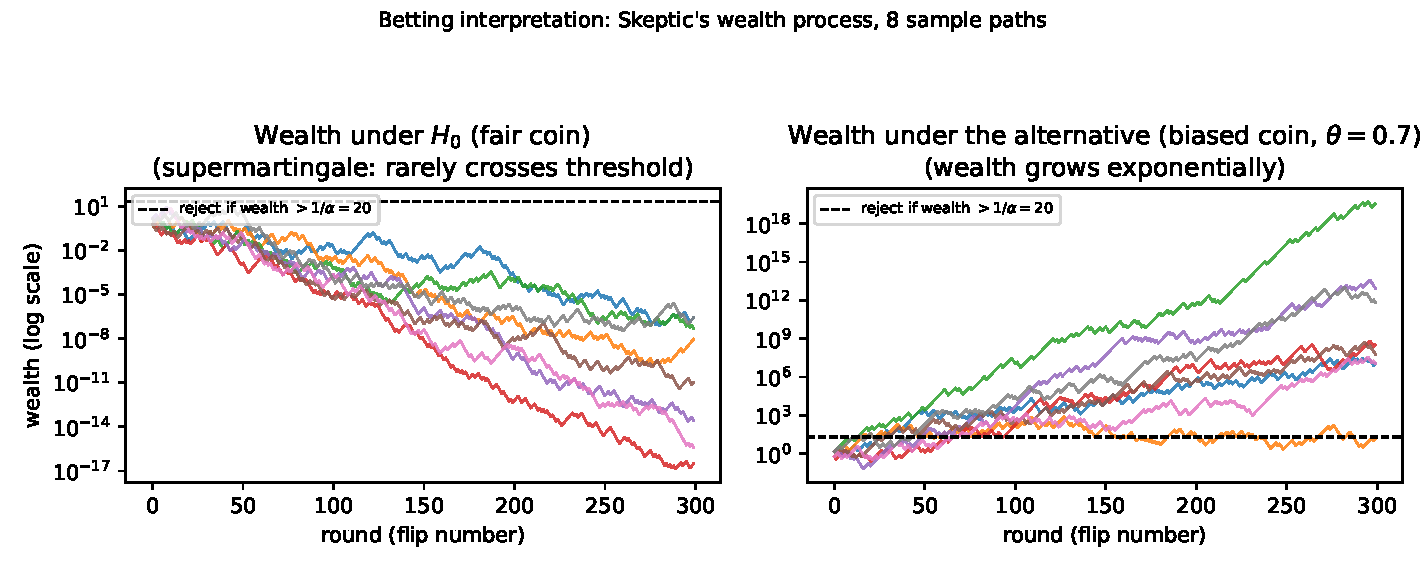
\includegraphics[width=0.98\textwidth]{fig_betting_wealth.pdf}

\vspace{0.3em}
\footnotesize
Eight simulated wealth paths from repeatedly betting $E = (0.7/0.5)^{\text{heads}}(0.3/0.5)^{\text{tails}}$
per flip. \textbf{Left:} under the null ($\theta=0.5$), wealth fluctuates but
rarely exceeds the rejection threshold $1/\alpha$ (supermartingale intuition:
on average, wealth does not grow). \textbf{Right:} under the true
alternative ($\theta=0.7$), wealth grows exponentially -- Skeptic profits.
\end{frame}

\begin{frame}[fragile]{Python: Simulating the Wealth Process and Ville's Inequality}

\begin{lstlisting}
import numpy as np
rng = np.random.default_rng(2024)

alpha = 0.05
threshold = 1/alpha            # reject if wealth ever exceeds this
n_rounds = 300
n_reps = 5000
p0, q0 = 0.5, 0.7               # H0: fair coin; bet built against theta=0.7

max_wealth = np.zeros(n_reps)
for r in range(n_reps):
    flips = rng.binomial(1, p0, size=n_rounds)          # data under H0
    per_flip_e = np.where(flips == 1, q0/p0, (1-q0)/(1-p0))
    wealth = np.cumprod(per_flip_e)                     # running product = wealth
    max_wealth[r] = wealth.max()

frac_exceeds = np.mean(max_wealth > threshold)
print(f"P(max wealth over {n_rounds} rounds > 1/alpha={threshold:.0f}) = {frac_exceeds:.4f}")
print(f"Ville's inequality guarantees this is <= alpha = {alpha}")
\end{lstlisting}

\medskip
\textbf{Output:} \texttt{P(max wealth > 20) = 0.0490}, comfortably
respecting the $\le 0.05$ guarantee -- even though we checked the
\emph{running maximum} over all 300 rounds, not just the final value.
This is the practical payoff of the e-process property.

\end{frame}

%% ══════════════════════════════════════════════════════════════════════════
\section{1.6 A first example: likelihood ratio}
%% ══════════════════════════════════════════════════════════════════════════

\begin{frame}{1.6 A First Example: Likelihood Ratio}

The most natural e-variable of all: for testing a simple null $\mathbb{P}$
against a simple alternative $\mathbb{Q}\ll\mathbb{P}$ (reminder:
absolutely continuous, i.e., comparable densities), the likelihood ratio
itself is an e-variable.

\begin{block}{Likelihood-ratio e-variable}
\emph{Intuition:} how much more plausible is the data under $\mathbb{Q}$
than under $\mathbb{P}$? That ratio, applied to the observed data, is
automatically a valid (exact) e-value for $\mathbb{P}$.
\[
  E = \frac{\mathrm{d}\mathbb{Q}}{\mathrm{d}\mathbb{P}}(X).
\]
\begin{itemize}
  \item $X$: the observed data.
  \item For \emph{any} $\mathbb{Q}\ll\mathbb{P}$, this $E$ is an e-variable
    for $\mathbb{P}$, and in fact \emph{exact}
    ($\mathbb{E}^{\mathbb{P}}[E]=1$).
\end{itemize}
\end{block}

We specialize to two settings the book uses throughout: Gaussian mean
shift, and our running Bernoulli (coin flip) example.

\end{frame}

\begin{frame}{1.6 Likelihood Ratio: the Gaussian Example}
\small
\begin{block}{Gaussian example (Eq.\ 1.1--1.2)}
Testing $\mathbb{P}=\mathrm{N}(0,1)$ against $\mathbb{Q}=\mathrm{N}(\mu,1)$
($\mu>0$ known), with i.i.d.\ data $X_1,\dots,X_n$ and $S_n=\sum_i X_i$:
\[
  E_n = \exp\!\big(\mu S_n - n\mu^2/2\big) = \prod_{i=1}^n \exp(\mu X_i - \mu^2/2).
\]
\begin{itemize}
  \item $S_n$: sum of the $n$ observations.
  \item Each factor $\exp(\mu X_i-\mu^2/2)$ is itself an exact e-variable;
    their product remains exact ($\mathbb{E}^{\mathbb{P}}[E_n]=1$).
\end{itemize}
Writing $\delta=\mu\sqrt{n}$ (signal strength) and $Z=S_n/\sqrt{n}$
(standard normal under $H_0$):
\[
  E_n = \exp\!\big(\delta Z - \delta^2/2\big),
  \qquad
  P_n = \Phi(-S_n/\sqrt n) = \Phi(-Z)
\]
\begin{itemize}
  \item $\Phi$: standard normal cdf; $P_n$ is the classical Neyman--Pearson
    p-variable.
  \item $E_n$ increasing in $S_n$, $P_n$ decreasing in $S_n$: both agree
    that larger $S_n$ favors $\mathbb{Q}$.
\end{itemize}
\end{block}

\end{frame}

\begin{frame}{1.6 Likelihood Ratio: the Two-Sided Version}

\begin{block}{Two-sided version (Eq.\ 1.3--1.4)}
Testing $\mathrm{N}(0,1)$ against $\mathrm{N}(\mu,1)$ for \emph{unknown}
$\mu\neq 0$, using a free parameter $\delta>0$:
\[
  E_n = \frac{\exp(\delta Z - \delta^2/2) + \exp(-\delta Z - \delta^2/2)}{2},
  \qquad
  P_n = 2\Phi(-|Z|).
\]
\begin{itemize}
  \item Averaging the ``$+\mu$'' and ``$-\mu$'' bets (Fact 1.3(iii)) gives
    a valid e-variable for the two-sided problem.
  \item $\delta$ is a design choice affecting power -- addressed in later
    chapters.
\end{itemize}
\end{block}

\end{frame}

\begin{frame}{1.6 Likelihood Ratio: the Bernoulli (Coin-Flip) Version}

\begin{block}{Bernoulli / coin-flip version (Eq.\ 1.5) -- our running example}
Testing $\mathbb{P}=\mathrm{Bernoulli}(p)$ vs.\ $\mathbb{Q}=\mathrm{Bernoulli}(q)$,
$q>p$, sample size $n$, $S_n=\sum_i X_i$ (number of heads):
\[
  E_n = \left(\frac{q}{p}\right)^{S_n}\left(\frac{1-q}{1-p}\right)^{n-S_n}.
\]
\begin{itemize}
  \item $E_n$ exact, increasing in $S_n$; Neyman--Pearson p-variable is
    $P_n = 1 - F_{n,p}(S_n)$ (upper binomial tail).
  \item This is our \textbf{running example} for the rest of the deck:
    testing whether a coin is fair.
\end{itemize}
\end{block}

\end{frame}

\begin{frame}{Worked Example: Is Our Coin Fair? (Step by Step)}

\textbf{Setup.} $H_0:\theta=0.5$ (fair coin) vs.\ chosen alternative
$\theta=0.7$. We flip $n=20$ times and observe $S_{20}=14$ heads.

\begin{block}{Computing the e-value, one step at a time}
\begin{itemize}
  \item \textbf{Step 1} (identify the formula): use Eq.\ 1.5 with
    $p=0.5$, $q=0.7$, $n=20$, $S_n=14$.
  \item \textbf{Step 2} (plug in):
    $E_{20} = (0.7/0.5)^{14}\,(0.3/0.5)^{6} = (1.4)^{14}(0.6)^{6}$.
  \item \textbf{Step 3} (compute each factor):
    $1.4^{14} \approx 111.12$, \quad $0.6^{6} = 0.046656$.
  \item \textbf{Step 4} (multiply):
    $E_{20} \approx 111.12 \times 0.046656 \approx 5.18$.
  \item \textbf{Step 5} (interpret): $E_{20}\approx 5.18 > 1$ is mild
    evidence \emph{against} the fair-coin null -- but well below
    $1/\alpha = 20$ for $\alpha=0.05$, so we would \emph{not} reject at
    that level.
\end{itemize}
\end{block}

\textbf{For comparison}, the exact one-sided p-value is
$P(S_{20}\ge 14\mid\theta=0.5) \approx 0.058$ -- also not significant at
$\alpha=0.05$, consistent with the e-value's verdict.

\end{frame}

\begin{frame}[allowframebreaks]{Example 1.4: Unknown Sampling Scheme}

This is the book's own example illustrating why e-values tolerate unknown
data-collection designs, while p-values do not.

\begin{block}{Setup}
Testing $\mathbb{P}=\mathrm{Bernoulli}(1/2)$ vs.\ $\mathbb{Q}=\mathrm{Bernoulli}(q)$,
$q>1/2$. A scientist is handed the dataset $(1,1,0,1,1,1,1,1)$ -- 8 points,
7 heads -- \emph{without} being told how it was collected.
\begin{itemize}
  \item \textbf{Design (a):} collect exactly 8 points.
    P-value $= \mathbb{P}(N_8\ge 7) = 0.035$ (significant at 0.05).
  \item \textbf{Design (b):} collect data until 5 heads occur in a row.
    P-value $= \mathbb{P}(\text{5-in-a-row observed at or before } n=8) = 0.078$
    (\emph{not} significant at 0.05).
\end{itemize}
\end{block}

\framebreak

\begin{itemize}
  \item \textbf{The problem:} if only the data (not the design) is
    reported, the scientist cannot tell whether they're in case (a), (b),
    or some other design -- yet the p-value's validity crucially depends
    on knowing which.
  \item \textbf{The fix:} the e-value
    $E_n = q^{S_n}(1-q)^{n-S_n}/2^n$ from Eq.\ 1.5 (with $p=1/2$) remains a
    \emph{valid} e-variable \textbf{regardless of the data-collecting
    design}, as long as all obtained data is used from the start.
  \item \textbf{Why:} $(E_n)_{n\ge1}$ forms an e-process (Chapter 7) -- it
    stays valid at any data-dependent stopping rule, which is exactly the
    ``no peeking into the future'' property from the notation frame.
  \item \textbf{Caveat:} this does not rescue \emph{malicious} designs
    (cherry-picking only 1s, discarding early 0s, reporting only the ``best''
    of several batches) -- no statistical method purely based on collected
    data can fix that.
\end{itemize}

\end{frame}

\begin{frame}{Figure: P-values vs.\ E-values Under Repeated Null Experiments}
\centering
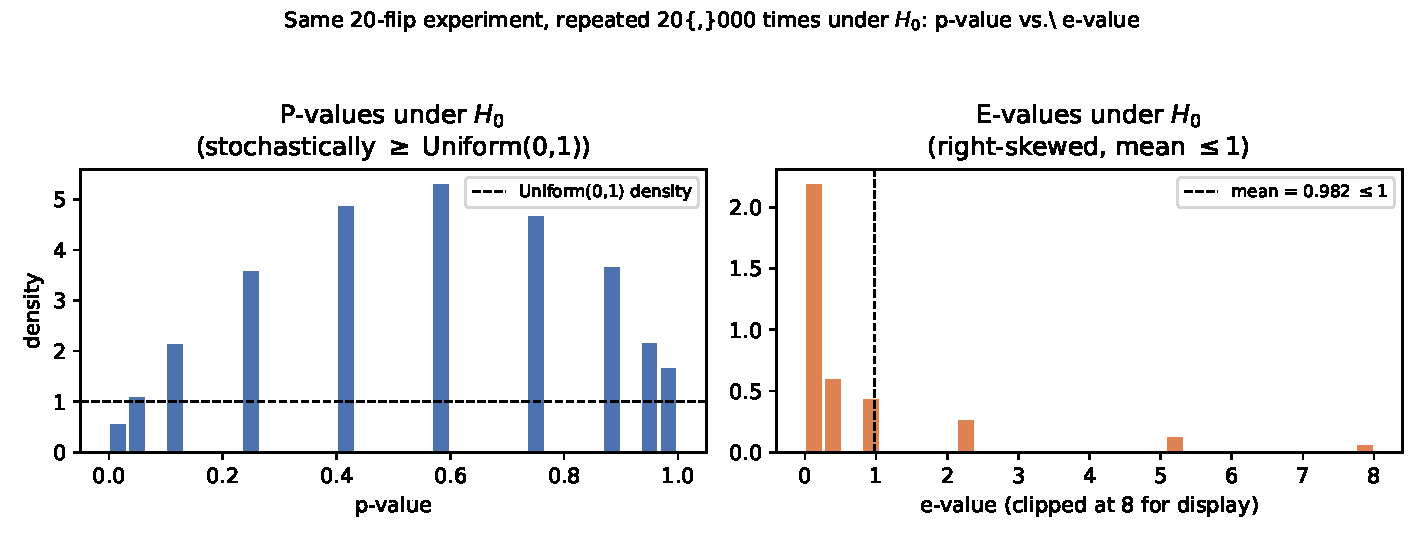
\includegraphics[width=0.98\textwidth]{fig_pvalue_vs_evalue_hist.pdf}

\vspace{0.3em}
\footnotesize
20{,}000 simulated repeats of our $n=20$ coin-flip experiment under
$H_0:\theta=0.5$. \textbf{Left:} p-values are (stochastically) uniform on
$[0,1]$ -- as required by the p-variable definition. \textbf{Right:}
e-values are right-skewed (most realizations are modest or small, a few
are large) with sample mean $\approx 0.98\le 1$, exactly as the e-variable
definition demands. Numerically, $\mathbb{P}(E>20)\approx 0.006 \le 1/20$,
confirming Markov's inequality.
\end{frame}

\begin{frame}[allowframebreaks]{An Illustration: Sequential Data and Adaptive Strategies}

Suppose data $X_1,\dots,X_n$ from parameter $\theta^{\dagger}$ arrive one
at a time, testing $H_0:\theta^{\dagger}=0$ vs.\ $H_1:\theta^{\dagger}\in\Theta_1$.
Let $\ell(x;\theta)=\mathrm{d}\mathbb{Q}_\theta/\mathrm{d}\mathbb{P}(x)$. Any
choice of $\theta$ turns $\ell(X_i;\theta)$ into a valid e-variable for
$H_0$ -- so we have freedom in how to pick $\theta$ at each step:
\begin{itemize}
  \item[(a)] \textbf{Fixed}: pick $\theta_1,\dots,\theta_n\in\Theta_1$ in
    advance (possibly all equal).
  \item[(b)] \textbf{Adaptive}: estimate $\theta_k$ from
    $X_1,\dots,X_{k-1}$ only -- e.g., via maximum likelihood (MLE) or
    maximum a posteriori (MAP).
\end{itemize}

\framebreak

\begin{block}{The running product is always a valid martingale}
\emph{Intuition:} no matter how cleverly (or adaptively) you pick each
$\theta_i$, as long as you only use \emph{past} data to do so, multiplying
per-round e-variables together keeps you honest -- your expected next-step
wealth, given everything so far, is exactly your current wealth.

Define $M_n := \prod_{i=1}^n E_i$ with $E_i=\ell(X_i;\theta_i)$, $M_0=1$.
\[
  \mathbb{E}^{\mathbb{P}}\!\big[M_i \mid X_1,\dots,X_{i-1}\big]
  = M_{i-1}\cdot\mathbb{E}^{\mathbb{P}}\!\big[\ell(X_i;\theta_i)\mid X_1,\dots,X_{i-1}\big]
  = M_{i-1}.
\]
\begin{itemize}
  \item \textbf{Step 1}: factor $M_i = M_{i-1}\cdot E_i$ out of the
    conditional expectation ($M_{i-1}$ is already known given the past).
  \item \textbf{Step 2}: $\theta_i$ is computed from
    $X_1,\dots,X_{i-1}$ only, so $\mathbb{E}^{\mathbb{P}}[\ell(X_i;\theta_i)\mid X_1,\dots,X_{i-1}]=1$
    (it's an exact e-variable given the past).
  \item \textbf{Conclusion}: $(M_i)$ never grows \emph{on average} given
    the past -- the martingale/supermartingale property from the notation
    frame.
\end{itemize}
\end{block}

\framebreak

\textbf{Example 1.5 (book):} data from $\mathrm{N}(\theta^\dagger,1)$ with
true $\theta^\dagger=0.3$; $H_0:\theta^\dagger=0$. Six strategies for
choosing $\theta_i$: (i) true value $0.3$ (log-optimal); (ii) misspecified
$0.1$; (iii) random, $\theta_i\sim\mathrm{Unif}[0,0.5]$ i.i.d.; (iv) MAP
with prior $\mathrm{N}(0.1,0.2^2)$; (v) MLE from $X_1,\dots,X_{i-1}$
(started at $\theta_1=0.1$); (vi) discrete mixture over a uniform grid on
$[0,0.6]$. For large $n$, methods (iv), (v), (vi) grow \emph{almost as
fast} as the (unrealistic, oracle) method (i); misspecified/random
strategies (ii), (iii) grow more slowly.

\framebreak

\centering
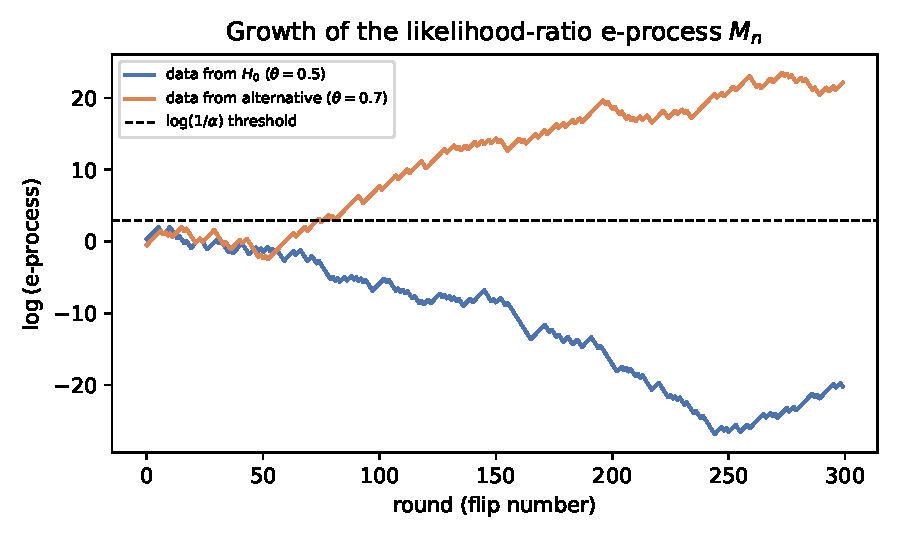
\includegraphics[width=0.62\textwidth]{fig_eprocess_growth.pdf}

\footnotesize
Our own simplified illustration in the same spirit: a single e-process
run under $H_0$ (bounded, rarely crosses the $1/\alpha$ threshold) versus
under the true alternative (grows essentially linearly in log-scale, i.e.
exponentially).

\end{frame}

\begin{frame}[fragile]{Python: 1000 Replications --- Confirming Mean E-value $\le 1$}

\begin{lstlisting}
import numpy as np
rng = np.random.default_rng(3)

n, p0, q0 = 20, 0.5, 0.7
n_reps = 1000
S = rng.binomial(n, p0, size=n_reps)          # simulate data under H0, 1000 times
E = (q0/p0)**S * ((1-q0)/(1-p0))**(n-S)        # e-value for each replication

print("Sample mean of E over 1000 replications:", E.mean())
print("Sample max of E:", E.max())
print("Fraction with E > 1/0.05 = 20:", np.mean(E > 20))

# The one specific dataset we highlighted in the worked example:
S_obs = 14
E_obs = (q0/p0)**S_obs * ((1-q0)/(1-p0))**(n-S_obs)
print("E for our observed 14-heads-out-of-20 dataset:", round(E_obs, 4))
\end{lstlisting}

\medskip
\textbf{Output (excerpt):} \texttt{Sample mean of E $\approx$ 0.99}
(consistent with the $\le 1$ guarantee up to Monte Carlo error),
\texttt{Fraction with E > 20 $\approx$ 0.005--0.01} ($\le 0.05$, as Markov's
inequality demands), and \texttt{E for our observed dataset = 5.1844},
matching the hand computation on the previous slide.

\end{frame}

%% ══════════════════════════════════════════════════════════════════════════
\section{1.7 A second example: the soft-rank e-value}
%% ══════════════════════════════════════════════════════════════════════════

\begin{frame}{1.7 A Second Example: The Soft-Rank E-value}

Many classical procedures (permutation tests, Monte Carlo tests) produce
statistics that are \emph{exchangeable} under the null (reminder: their
joint distribution is unchanged by relabeling) and use the \emph{rank} of
the real statistic among simulated copies as a p-value. This section
converts that idea into an e-value.

\begin{block}{Setup}
\emph{Intuition:} we have one real test statistic $L_0$ and $B$
``fake'' copies $L_1,\dots,L_B$ that look statistically identical to $L_0$
under the null (e.g., generated by random permutations). We want to turn
the comparison ``is $L_0$ unusually large?'' into a valid e-value.
\begin{itemize}
  \item $L_0$: statistic from the real data (larger = more evidence
    against $H_0$).
  \item $L_1,\dots,L_B$: $B$ additional statistics, exchangeable together
    with $L_0$ under $\mathcal{P}$.
  \item \textbf{Example source of exchangeability}: testing independence
    of paired data $(X_i,Y_i)$ via sample correlation $L_0$; permute the
    $X$'s randomly $B$ times to get $L_1,\dots,L_B$.
\end{itemize}
\end{block}

\end{frame}

\begin{frame}{The Soft-Rank E-value Formula}

\begin{block}{Definition (soft-rank e-value)}
First transform $L_0,\dots,L_B$ into nonnegative scores
$R_0,\dots,R_B$ that preserve their order and exchangeability (details
next slide), then define
\[
  E = \frac{(B+1)R_0}{\sum_{b=0}^B R_b}
  \qquad (\text{with } E:=1 \text{ if } \textstyle\sum_b R_b = 0).
\]
\begin{itemize}
  \item $R_0$: the transformed score of the \emph{real} data's statistic.
  \item $\sum_{b=0}^B R_b$: total score across the real statistic and all
    $B$ exchangeable copies.
  \item \emph{Why this is an e-variable:} by exchangeability of
    $R_0,\dots,R_B$ under $\mathcal{P}$, one can show
    $\mathbb{E}^{\mathbb{P}}\!\big[R_0 \,\big|\, \textstyle\sum_b R_b\big] = \frac{\sum_b R_b}{B+1}$,
    which after rearranging gives $\mathbb{E}^{\mathbb{P}}[E]=1$ (exact).
\end{itemize}
\end{block}

\end{frame}

\begin{frame}{Example 1.7: A Concrete Score Transformation}

\begin{block}{Example 1.7: one concrete transformation}
For a constant $r>0$ and $L_*=\min_{b} L_b$:
\[
  R_b = \frac{\exp(rL_b) - \exp(rL_*)}{r} \;\ge 0.
\]
\begin{itemize}
  \item As $r\to 0$: $R_b \to L_b - L_*\ge 0$ (a simple shift).
  \item If the $L_b$ are already nonnegative, the simplest valid choice is
    $r=0$ with $L_*=0$, i.e., \textbf{just use $R_b=L_b$ directly}.
\end{itemize}
\end{block}

\end{frame}

\begin{frame}{Concrete Numbers: Soft-Rank E-value on Our Coin Data}

\small
We instantiate the abstract machinery with our own 20-flip dataset (14
heads), using the \textbf{longest run of heads} as the test statistic
(a classic way to check whether a sequence looks ``too streaky'' to be a
fair, independent coin).

\begin{block}{Step-by-step calculation}
\begin{itemize}
  \item \textbf{Data:} \texttt{1101110101010101 0111} (14 heads, 6 tails,
    engineered with a run of 6 heads at the start).
  \item \textbf{Step 1:} compute $L_0 = $ longest head-run in the original
    data $= 6$.
  \item \textbf{Step 2:} draw $B=4$ independent random permutations of the
    same 20 flips; compute longest head-runs
    $L_1,\dots,L_4 = 7,\,5,\,4,\,5$.
  \item \textbf{Step 3:} since all $L_b\ge 0$, take $R_b=L_b$ (the $r=0$
    choice). So $R_0,\dots,R_4 = 6,7,5,4,5$, summing to $27$.
  \item \textbf{Step 4:} soft-rank e-value
    $E = \dfrac{(4+1)\times 6}{27} = \dfrac{30}{27} \approx 1.111$.
  \item \textbf{Step 5:} ordinary permutation p-value
    $P = \dfrac{\#\{b: L_b\ge L_0\}}{B+1} = \dfrac{2}{5} = 0.4$
    (namely $b=0,1$ tie/exceed $L_0=6$).
  \item \textbf{Check the book's inequality} $P\le 1/E$:
    indeed $0.4 \le 1/1.111 = 0.9$. \checkmark
\end{itemize}
\end{block}

\end{frame}

\begin{frame}[fragile]{Python: Computing the Soft-Rank E-value}

\begin{lstlisting}
import numpy as np
def longest_run(seq, val=1):
    best = cur = 0
    for x in seq:
        cur = cur + 1 if x == val else 0
        best = max(best, cur)
    return best

seq = [1,1,1,1,1,1,0,1,0,1,0,1,0,1,0,1,0,1,1,1]  # 20-flip data, 14 heads
L0 = longest_run(seq)
rng = np.random.default_rng(11)
B = 4
Ls = [L0] + [longest_run(list(rng.permutation(seq))) for _ in range(B)]
R = np.array(Ls, dtype=float)          # r=0 choice: R_b = L_b (nonnegative)
E = (B + 1) * R[0] / R.sum()
P = np.mean(np.array(Ls) >= L0)        # ordinary permutation p-value
print("L_0..L_4 =", Ls, " E =", round(E,4), " P =", P, " P<=1/E:", P <= 1/E)
\end{lstlisting}

\medskip
\textbf{Output:} \texttt{L\_0..L\_4 = [6, 7, 5, 4, 5]},
\texttt{E = 1.1111}, \texttt{P = 0.4}, \texttt{P<=1/E: True}
($0.4 \le 0.9$) -- matching the hand calculation exactly.

\end{frame}

\begin{frame}{Why ``Soft-Rank''?}

\begin{itemize}
  \item The usual permutation p-value only looks at the \emph{rank} of
    $L_0$ among $L_0,\dots,L_B$: $P = \sum_b \mathbf{1}\{L_b\ge L_0\}/(B+1)$.
  \item After the exponential-style transform, $1/E$ can be seen as a
    ``smoothed'' version of that rank -- hence \textbf{soft-rank p-value}
    for $1/E$, and \textbf{soft-rank e-value} for $E$ (analogous to how
    ``soft-max'' smooths the maximum via exponentiation).
  \item The book shows algebraically that $P \le 1/E$ always -- the direct
    p-value is never larger than the soft-rank p-value, so at first glance
    there's no advantage to using $E$ for a \emph{single} test.
  \item \textbf{But:} Chapters 8--11 show e-values enjoy real advantages
    over p-values specifically in multiple testing and building confidence
    intervals -- advantages invisible when testing just one hypothesis.
\end{itemize}

\end{frame}

%% ══════════════════════════════════════════════════════════════════════════
\section{1.8 Historical context}
%% ══════════════════════════════════════════════════════════════════════════

\begin{frame}[allowframebreaks]{1.8 Historical Context: Who Invented E-values?}

\textbf{Short answer: nobody, and everybody.} If $\mathcal{P}=\{\mathbb{P}\}$
is simple, every optimal e-value is (or is dominated by) a likelihood
ratio -- and likelihood ratios are $\sim$100 years old, central to both
frequentist and Bayesian statistics. What's new is recognizing e-values as
a \emph{general, composite-hypothesis-friendly} concept and the coordinated
choice of the term ``e-value'' itself (agreed jointly by researchers in
2020).

\medskip
The book credits five central historical figures, in chronological order:

\begin{itemize}
  \item \textbf{Ville (1939):} brought (nonnegative) martingales to the
    center of probability theory; showed any measure-zero event has a
    nonnegative martingale exploding to $\infty$ on it. Motivated by
    critiquing von Mises' theory of ``collectives,'' not statistical
    inference per se.
  \item \textbf{Wald (1945):} invented sequential analysis; nonnegative
    martingales (esp.\ the likelihood-ratio process) are central to his
    sequential probability ratio test, though framed around a single
    pre-specified stopping time.
\end{itemize}

\framebreak

\begin{itemize}
  \item \textbf{Kelly (1956):} proposed \emph{log-optimality} -- betting to
    maximize the expected log-growth rate of wealth in repeated favorable
    games, linking gambling to Shannon's information theory. (Breiman,
    1961, generalized this beyond binary outcomes.)
  \item \textbf{Robbins (1970, with Darling 1967):} defined confidence
    sequences and ``power-one'' tests; recognized that products of
    e-values yield nonnegative supermartingales, and pushed for
    \emph{anytime-valid} inference rather than Wald's fixed stopping rule.
  \item \textbf{Cover (1984):} developed log-optimal portfolio theory for
    financial trading with regret bounds against the best fixed portfolio
    in hindsight -- a close cousin of log-optimal e-values.
\end{itemize}

\medskip
\textbf{Vovk} later spearheaded the modern \emph{game-theoretic
probability} program (from 1993 onward, with Shafer and others),
culminating in the term ``e-value'' being jointly adopted by Vovk, Shafer,
Grünwald, Ramdas, and Wang around 2020.

\end{frame}

\begin{frame}[allowframebreaks]{Recent Progress: The 2018--2020 Explosion}

A remarkable concentration of independent, aligned papers appeared on
arXiv within a two-year window:

\begin{itemize}
  \item \textbf{2018 (Howard, Ramdas, McAuliffe, Sekhon):} e-processes via
    families of supermartingales + Ville's inequality $\Rightarrow$
    nonparametric confidence sequences.
  \item \textbf{2018 (Kaufmann \& Koolen):} mixture method for likelihood
    ratios in exponential families; sequential KL-divergence bounds.
  \item \textbf{2019 (Shafer):} expository case for betting-based
    scientific communication and log-optimality.
  \item \textbf{2019 (Shafer \& Vovk, book):} game-theoretic foundations of
    probability and finance.
  \item \textbf{2019 (Grünwald, De Heide, Koolen):} simpler e-process
    definition (valid at any stopping time); reverse information
    projection; meta-analysis applications.
\end{itemize}

\framebreak

\begin{itemize}
  \item \textbf{2019 (Vovk \& Wang):} averaging is essentially the
    \emph{only} admissible way to combine dependent e-values; e-to-p and
    p-to-e calibrators. This paper triggered the community-wide agreement
    on the term ``e-value.''
  \item \textbf{2019 (Wasserman, Ramdas, Balakrishnan):} ``universal
    inference'' -- e-values from split-likelihood-ratio statistics, valid
    with zero regularity conditions.
  \item \textbf{2020 (Vovk, Wang, Wang):} admissible p-value merging must
    go through e-values (via optimal transport duality).
  \item \textbf{2020 (Wang \& Ramdas):} e-BH, an e-value analogue of
    Benjamini--Hochberg, controlling FDR under \emph{arbitrary} dependence.
  \item \textbf{2020 (Ramdas, Ruf, Larsson, Koolen):} necessary and
    sufficient conditions for admissible SAVI (sequential anytime-valid
    inference) tools.
  \item \textbf{2020 (Waudby-Smith \& Ramdas):} testing-by-betting for
    bounded-mean estimation; universal representation of nonnegative
    martingales.
\end{itemize}

\end{frame}

\begin{frame}{Unfortunate Name Clashes: Other ``E-values'' in the Wild}

The letter ``e'' was popular before this book -- watch out for these
unrelated uses of ``E-value'' in other literatures:

\begin{itemize}
  \item \textbf{BLAST E-value} (bioinformatics): expected number of chance
    hits in a sequence database; roughly $E=-\log(1-P)$ applied to a
    p-value -- a different object entirely.
  \item \textbf{Sensitivity E-value} (VanderWeele \& Ding, 2017, causal
    inference): the minimum confounding strength (on a risk-ratio scale)
    needed to fully explain away an observed association.
  \item \textbf{Bayesian E-value} (Pereira \& Stern, 1999): the
    \emph{epistemic} value $ev(H\mid X)$ in the Full Bayesian Significance
    Test -- a Bayesian evidence measure, unrelated to this book's
    expectation-based definition.
\end{itemize}

\medskip
Reassuringly, the terms ``e-variable'' and ``e-process'' have no known
clashes -- use them alongside ``e-value'' when precision matters.

\end{frame}

%% ══════════════════════════════════════════════════════════════════════════
\section{1.9 Road map}
%% ══════════════════════════════════════════════════════════════════════════

\begin{frame}[allowframebreaks]{1.9 Road Map of the Book}

The book is organized into three parts, building from foundations to
advanced applications.

\begin{block}{Part I: Fundamental Concepts (Ch.\ 1--4)}
\begin{itemize}
  \item \textbf{Ch.\ 2 --- Validity.} Properties of e-values under the
    null: Markov's inequality, calibrators, randomized tests; explicit
    e-variables in simple examples.
  \item \textbf{Ch.\ 3 --- Efficiency.} Properties under the alternative:
    e-power, log-optimality, existence of powered e-values, mixture/plug-in
    methods.
  \item \textbf{Ch.\ 4 --- Post-hoc decisions.} E-values' role when parts
    of the testing problem (level, decisions, or even data collection)
    depend on the data itself.
\end{itemize}
\end{block}

\framebreak

\begin{block}{Part II: Core Ideas (Ch.\ 5--9)}
\begin{itemize}
  \item \textbf{Ch.\ 5 --- Universal inference:} a simple, general method
    for building e-variables for composite nulls/alternatives -- the first
    known test for many ``irregular'' problems (though improvable).
  \item \textbf{Ch.\ 6 --- Log-optimal e-variables:} a unique
    ``numeraire'' e-variable always exists for a fixed alternative,
    connected to the reverse information projection.
  \item \textbf{Ch.\ 7 --- SAVI:} sequential anytime-valid inference --
    e-processes, testing by betting, optional stopping, Ville's inequality.
  \item \textbf{Ch.\ 8 --- Merging e-values:} combining via averages
    (arbitrary dependence) or products (independence).
  \item \textbf{Ch.\ 9 --- Compound e-values:} e-Benjamini--Hochberg for
    false discovery rate control.
\end{itemize}
\end{block}

\framebreak

\begin{block}{Part III: Advanced Topics (Ch.\ 10--16)}
\begin{itemize}
  \item \textbf{Ch.\ 10:} approximate/asymptotic e- and p-values.
  \item \textbf{Ch.\ 11:} combining dependent e-values is only admissible
    via (weighted) averaging.
  \item \textbf{Ch.\ 12:} combining dependent p-values (via e-values and
    optimal transport duality).
  \item \textbf{Ch.\ 13:} e-confidence intervals; e-Benjamini--Yekutieli
    for false coverage rate.
  \item \textbf{Ch.\ 14:} further e-value/p-value contrasts and dualities.
  \item \textbf{Ch.\ 15:} improved (sub-$1/\alpha$) thresholds under shape
    or dependence assumptions.
  \item \textbf{Ch.\ 16:} connections to risk measures; nonparametric tests
    for forecasts.
\end{itemize}
\end{block}

\framebreak

\begin{block}{Four cross-cutting goals}
\begin{enumerate}
  \item \textbf{Understanding the foundations:} Chapters 2, 4, 10, 14.
  \item \textbf{Constructing good/powerful e-values:} Chapters 3, 6, 15.
  \item \textbf{Designing inference methods:} Chapters 5, 7, 16.
  \item \textbf{Designing multiple-testing methods:} Chapters 8, 9, 11,
    12, 13.
\end{enumerate}
\end{block}

In the first two categories, the object of interest is the e-value
\emph{itself}; in the remaining two, the e-value is a means to a specific
statistical end.

\end{frame}

%% ══════════════════════════════════════════════════════════════════════════
\section{Summary}
%% ══════════════════════════════════════════════════════════════════════════

\begin{frame}{Chapter 1 --- Key Takeaways}

\begin{itemize}
  \item An \textbf{e-value} is a nonnegative statistic with expectation
    $\le 1$ under the null -- a valid bet against $H_0$; large values are
    evidence against the null (opposite convention from p-values).
  \item E-values and p-values are \textbf{statistical cousins}: convertible
    via $P=1/E$ and $E=\mathbf{1}\{P\le\alpha\}/\alpha$, but e-values
    uniquely support post-hoc levels, optional continuation (via simple
    multiplication), and unknown sampling schemes.
  \item The preferred optimality criterion is \textbf{e-power}
    $\mathbb{E}^{\mathbb{Q}}[\log E]$, forced by the algebra of repeatedly
    multiplying e-values together.
  \item The \textbf{betting interpretation} (Forecaster vs.\ Skeptic) is
    the intuitive engine behind the whole framework: e-variables are
    exactly the wealth-generating bets Forecaster would accept.
  \item Two worked templates recur throughout the book: the
    \textbf{likelihood-ratio e-value} (our coin example: $n=20$, $14$
    heads, $E\approx 5.18$) and the \textbf{soft-rank e-value}
    (permutation-style tests, our longest-run example: $E\approx 1.11$).
  \item Five names anchor the history: \textbf{Ville, Wald, Kelly, Robbins,
    Cover} -- with Vovk, Shafer, Grünwald, Ramdas, and Wang driving the
    modern synthesis.
  \item The rest of the book builds outward from these definitions:
    validity (Ch.\ 2), efficiency (Ch.\ 3), post-hoc decisions (Ch.\ 4),
    and onward through sequential and multiple-testing applications.
\end{itemize}

\end{frame}

\end{document}
